\documentclass[11pt,letterpaper]{article}
\usepackage[margin=.72in,top=.73in,bottom=.70in,headheight=15pt,headsep=15pt,footskip=25pt]{geometry}
\usepackage[T1]{fontenc}\usepackage{lmodern}
\usepackage{amsmath,amssymb,tikz,array,fancyhdr,hyperref}
\usetikzlibrary{arrows.meta}
\hypersetup{colorlinks=true,urlcolor=blue}
\renewcommand{\familydefault}{\sfdefault}
\pagestyle{fancy}\fancyhf{}
\fancyhead[L]{\small Week 71 / Can you hear the room? / Adult guide}
\fancyfoot[L]{\scriptsize Bellingham Math Circle / Week 71 / GGT71-FAC-v1}
\fancyfoot[R]{\scriptsize\thepage}
\renewcommand{\headrulewidth}{.3pt}\renewcommand{\footrulewidth}{0pt}
\setlength{\parindent}{0pt}\setlength{\parskip}{7pt}
\newcommand{\sectiontitle}[1]{\par\vspace{4pt}{\large\bfseries #1}\par}
\newcommand{\answer}[1]{\par\vspace{3pt}\textbf{Problem #1.} }
\begin{document}
\sectiontitle{The mathematics first}
\textbf{Bounce words can distinguish some rooms, but no word distinguishes two labeled rectangles.} A legal shot starts in the interior, travels straight between equal-angle reflections, and avoids corners for the observed segment. Its word records wall labels in order; lengths, times and starting point are not supplied.

With $A$ the bottom and $B$ the left side, \textbf{ABA is impossible in every rectangle}. After hitting $A$ the shot travels upward; hitting a vertical wall only reverses its horizontal motion. It cannot return to $A$ next. A $60^\circ$ rhombus \textbf{can} make ABA, as the checked example on page 2 shows.

\textbf{All rectangles have the same bounce words} when $A,B,C,D$ correspond to bottom, left, top, right. A positive horizontal/vertical stretch sends unfolded straight shots to straight shots, preserves their wall order, and preserves reflection in axis-parallel walls. The inverse stretch does the same. This is an all-word fact, not just an agreement among the examples.

\textbf{What children discover.} One valid drawing proves a word possible. Ruling out a room needs an impossibility argument; failed searching is insufficient. Several successful transfers suggest a rule, and the reversible stretch explains it. A finite observation need not reveal a unique room.

\textbf{Entry and depth.} This shared Grades 4--5 packet assumes children can trace a line across reflected copies and retain successive wall labels. The mirror step adds careful alignment and reflection. The universal rectangle argument is a later continuation; algebraic coordinates below are for adult checking, not a prerequisite for participation. The proposed age fit has not been classroom-tested.

\sectiontitle{Materials and the first visit}
\textbf{Per pair:} the five student pages, pencil/eraser, straightedge, a safe small mirror with a straight bottom edge, an opaque folder to hide shots, and spare copies or erasable sleeves of pages 1, 4 and 5. Print at actual size, without unequal-axis scaling. Page 5 contains two rhombus workspaces, each about $11.4$ cm wide and $6.58$ cm high; these are the precision surfaces, not the small page 3 candidate pictures.

At the older table, two children alternate drawing and checking while the third is a rotating referee. An adult should be available to check mirror placement. A mirror stands upright \emph{on} the wall, reflective face toward the room. The incoming segment should line up with the reflected image of the outgoing segment. No real ball, laser or aiming apparatus is needed.

\textbf{Common launch, about 5 minutes.} Let children look at a line in the mirror, then trace the printed AD example. In the side-$4$ square it goes from $(1,2)$ to $(3,0)$ on $A$, then to $(4,1)$ on $D$. The unfolded continuation crosses $D$ at $(4,-1)$ instead. Keep the starting dot and wall letters matched while a partner checks the same two hits.

\textbf{Manageable route:} allow 10--15 minutes to collect and check words in Problem 1, then investigate ABA in Problem 2. Play one Problem 3 round using an already checked drawing. That is a satisfying stopping point. The three mixed-wall transfers and all-word explanation in Problem 4 can form a return visit.

\textbf{Unrehearsed physical step.} Before use, try the AD check and a rhombus shot with the actual mirror and printouts. Verify its reflective edge is close enough to the paper and that partners can see the alignment. No such physical rehearsal or classroom pilot has occurred. If mirror alignment stalls, reuse the provided ABA unfolding and earlier checked shots rather than making the adult construct every new ray.
\newpage
\sectiontitle{Answers and optional hints}
\answer{1} Many six-word collections work. Here are six checked witnesses. For adult reconstruction, take the bold square as $[0,2]\times[0,2]$ and its starting dot as $(1,1)$. A direction $(u,v)$ means right $u$ and up $v$; negative values mean left/down. Draw the line through the listed third hit and stop there.
\begin{center}\renewcommand{\arraystretch}{1.25}
\begin{tabular}{@{}lll@{}}
Direction & First three wall letters & Third hit in the unfolded map\\\hline
$(3,2)$ & DCB & $(4,3)$\\
$(2,3)$ & CDA & $(3,4)$\\
$(-3,2)$ & BCD & $(-2,3)$\\
$(-2,3)$ & CBA & $(-1,4)$\\
$(-3,-2)$ & BAD & $(-2,-1)$\\
$(-2,-3)$ & ABC & $(-1,-2)$
\end{tabular}\end{center}
All stay within the page 1 window through their third hit and avoid corners. Accept other checked collections. A crossing through a vertex gives two walls at once and is not a legal word. \textit{Hint:} vary a successful line slightly, or reverse one component of its direction, and check what changes; do not hand out a memorized catalog.

\answer{2} \textbf{Square: no. Rhombus: yes.} The square impossibility follows from upward motion after $A$ surviving the $B$ bounce. Equivalently, in the supplied square unfolding a downward straight line cannot cross the horizontal line containing $A$ twice.

For a reproducible rhombus witness, use the side-$4$ room with vertices $(0,0),(4,0),(6,2\sqrt3),(2,2\sqrt3)$. Start at $(\frac{11}{4},\frac{\sqrt3}{4})$. The hits are
\[
 A:(2,0),\qquad B:(\tfrac12,\tfrac{\sqrt3}{2}),\qquad A:(2,0).
\]
\begin{center}
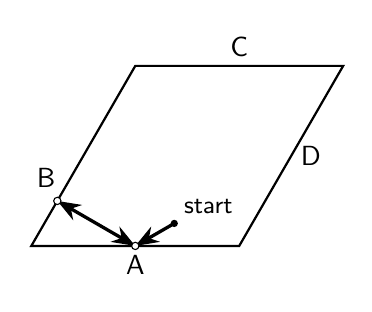
\begin{tikzpicture}[scale=.66]
\draw[thick](0,0)--(4,0)--(6,3.464101615)--(2,3.464101615)--cycle;
\node[below]at(2,0){A};\node[left]at(.65,1.30){B};\node[above]at(4,3.464101615){C};\node[right]at(5,1.732050808){D};
\fill(2.75,.433012702)circle(2pt);\node[above right,font=\small]at(2.75,.433012702){start};
\draw[very thick,-{Stealth}](2.75,.433012702)--(2,0);
\draw[very thick,{Stealth}-{Stealth}](2,0)--(.5,.866025404);
\draw[fill=white](2,0)circle(2pt);\draw[fill=white](.5,.866025404)circle(2pt);
\end{tikzpicture}
\end{center}
After the first $A$ reflection, the ray is perpendicular to $B$, so it reverses at $B$ and returns to the same $A$ point. Retracing is allowed; neither hit is a corner. In the printed unfolded chain the straight line hits $(2,0)$, $(\frac12,-\frac{\sqrt3}{2})$, then $(-1,-\sqrt3)$. All three hits are inside the intended wall segments.

\textit{Hint:} ``What happens when a shot meets a wall straight on?'' For transferring a child's different ray, use the mirror wall by wall; a plausible zigzag is not automatically a billiard shot.
\newpage
\sectiontitle{Secret-room play and the all-word conclusion}
\answer{3} Answers depend on the chosen word and the child's evidence. An \textbf{ABA} drawing rules out both rectangles by Problem 2, leaving the rhombus. A word already witnessed in a square is possible in the wide rectangle too. It may or may not be possible in the rhombus; keep the rhombus circled unless someone supplies a valid impossibility argument.

The entry is ``rooms not ruled out,'' not necessarily a complete list of rooms that mathematically realize the word. Require a checked witness for the secret room and a reason for each exclusion. On revealing the shot, audit the wall letters, equal-angle reflections and absence of corner hits. Use earlier checked drawings freely; new rhombus constructions are optional and use the large page 5 rooms.

\textit{Useful intervention:} ``Does not finding one yet show that nobody could draw one?'' A mistaken or corner-hitting secret shot should be repaired and replayed, not treated as evidence against a room.

\answer{4} \textbf{No bounce word can tell the square and wide rectangle apart.} Three legal mixed-wall examples within the supplied page 4 windows are DCB, CDA and BCD, using the first three rows of the page 2 table. Start at $(1,1)$ in the square and $(2,1)$ in the rectangle. Double each horizontal coordinate and leave vertical coordinates unchanged:
\begin{center}\renewcommand{\arraystretch}{1.25}
\begin{tabular}{@{}lll@{}}
Word & Square third hit & Wide-rectangle third hit\\\hline
DCB & $(4,3)$ & $(8,3)$\\
CDA & $(3,4)$ & $(6,4)$\\
BCD & $(-2,3)$ & $(-4,3)$
\end{tabular}\end{center}
The first, second and third hits all lie within the printed windows. Each example uses horizontal and vertical walls, as the task requires. The endpoints in this table are in the unfolded copies, not folded single-room coordinates.

\textbf{Why every word transfers.} Apply $(x,y)\mapsto(2x,y)$ to an entire unfolded picture. A straight line stays straight; each copied vertical/horizontal wall carries its old letter; crossings retain their order; non-corner crossings stay non-corner. Folding therefore produces a legal shot with the same word in the wide rectangle. Halving horizontal coordinates transfers any rectangle shot back to the square. This proves equality in both directions for all finite words, not just the three drawn.

More generally $(x,y)\mapsto(\alpha x,\beta y)$ works between any two rectangles when $\alpha,\beta>0$ and labels correspond. Reflection flips one velocity component; this commutes with coordinate stretching. Unequal stretching does \emph{not} generally preserve reflection at a sloping wall, so this argument does not show the rhombus has the same words.

\textit{Hint sequence:} compare where corresponding vertical and horizontal seams sit, then ask whether all points on one line can move together. Keep the stretch idea oral until children have made attempts.

\sectiontitle{Sources, checks, and limits}
Aaron Calderon, Solly Coles, Diana Davis, Justin Lanier and Andre Oliveira, \href{https://justinlanier.org/wp-content/uploads/2020/10/bounce.pdf}{\emph{How to hear the shape of a billiard table}} (2018): ABA comparison and Figure~2, p.~4; Proposition~1.6 and Corollary~1.7, p.~6. These supply the mathematical lineage, not this exact worksheet.

Moon Duchin, Viveka Erlandsson, Christopher J.~Leininger and Chandrika Sadanand, \href{https://arxiv.org/pdf/1804.05690}{\emph{You can hear the shape of a billiard table}}: Bounce Theorem, pp.~2--3. This is broader rigidity context; the children's finite experiments do not prove it.

The independent checker verifies the printed example coordinates, non-corner witnesses, exact rhombus reflection and rectangle transfers. The all-word claim rests on the stretch proof. This guide matches five-page GGT71-S-v1: four investigations plus reusable apparatus. Digitally checked and unpiloted; physical mirror work remains unrehearsed.
\end{document}
